\documentclass[10pt, aspectratio=169]{beamer}

% --- Packages ---
\usepackage{amsmath, amssymb, amsthm, mathtools}
\usepackage{booktabs}
\usepackage{tikz}
\usetikzlibrary{calc, positioning, shapes.geometric, arrows.meta}
\usepackage[most]{tcolorbox}
\usepackage{colortbl}

% --- Color Palette ---
\definecolor{navy}{RGB}{30,41,59}       % #1E293B Primary Dark Slate
\definecolor{teal}{RGB}{14,116,144}     % #0E7490 Primary Accent Teal
\definecolor{amber}{RGB}{217,119,6}     % #D97706 Highlight Warm Amber
\definecolor{slate}{RGB}{100,116,139}   % #64748B Secondary Muted
\definecolor{bglight}{RGB}{248,250,252} % #F8FAFC Background Light
\definecolor{cardbg}{RGB}{241,245,249}  % #F1F5F9 Box Fill
\definecolor{cardborder}{RGB}{226,232,240} % #E2E8F0 Border
\definecolor{darktext}{RGB}{15,23,42}   % #0F172A Text Dark

% --- Beamer Theme Customization ---
\setbeamercolor{background canvas}{bg=bglight}
\setbeamercolor{normal text}{fg=darktext}
\setbeamercolor{frametitle}{fg=navy, bg=bglight}
\setbeamercolor{title}{fg=navy}
\setbeamercolor{subtitle}{fg=teal}
\setbeamercolor{author}{fg=slate}
\setbeamercolor{date}{fg=slate}

% Remove default navigation symbols
\setbeamertemplate{navigation symbols}{}

% Clean Minimalist Frame Title
\makeatletter
\setbeamertemplate{frametitle}{
  \vspace*{0.15cm}
  \begin{beamercolorbox}[wd=\paperwidth, ht=0.85cm, dp=0.15cm, leftskip=0.8cm, rightskip=0.8cm]{frametitle}
    \usebeamerfont{frametitle}{\color{navy}\bfseries\insertframetitle}
    \ifx\insertframesubtitle\@empty\else
      \par\vspace*{1pt}
      {\usebeamerfont{framesubtitle}{\color{teal}\small\insertframesubtitle}}
    \fi
  \end{beamercolorbox}
  \vspace*{-0.1cm}
}
\makeatother

% Minimalist Footline
\setbeamertemplate{footline}{
  \begin{beamercolorbox}[wd=\paperwidth, ht=0.5cm, dp=0.2cm, leftskip=0.8cm, rightskip=0.8cm]{footline}
    {\color{slate}\tiny Nexa Institute of Technology \quad|\quad Lecture 7: The Spectral Theorem}
    \hfill
    {\color{teal}\bfseries\insertframenumber\,/\,\inserttotalframenumber}
  \end{beamercolorbox}
}

% Custom Styled Boxes with tcolorbox
\newtcolorbox{mathdef}[1]{
  enhanced,
  colback=cardbg,
  colframe=teal,
  arc=3pt,
  outer arc=3pt,
  boxrule=0.8pt,
  left=8pt, right=8pt, top=4pt, bottom=4pt,
  title={\bfseries\color{teal}\small #1},
  coltitle=teal,
  attach title to upper,
  after title={\par\vspace{2pt}\hrule height 0.4pt color teal!30\vspace{3pt}}
}

\newtcolorbox{maththeorem}[1]{
  enhanced,
  colback=cardbg,
  colframe=navy,
  arc=3pt,
  outer arc=3pt,
  boxrule=0.8pt,
  left=8pt, right=8pt, top=4pt, bottom=4pt,
  title={\bfseries\color{navy}\small #1},
  coltitle=navy,
  attach title to upper,
  after title={\par\vspace{2pt}\hrule height 0.4pt color navy!30\vspace{3pt}}
}

\newtcolorbox{proofstep}[1]{
  enhanced,
  colback=amber!5,
  colframe=amber,
  arc=3pt,
  outer arc=3pt,
  boxrule=0.8pt,
  left=8pt, right=8pt, top=4pt, bottom=4pt,
  title={\bfseries\color{amber}\small #1},
  coltitle=amber,
  attach title to upper,
  after title={\par\vspace{2pt}\hrule height 0.4pt color amber!40\vspace{3pt}}
}

\newtcolorbox{conceptbox}[1]{
  enhanced,
  colback=cardbg,
  colframe=cardborder,
  arc=3pt,
  outer arc=3pt,
  boxrule=0.6pt,
  left=8pt, right=8pt, top=4pt, bottom=4pt,
  title={\bfseries\color{navy}\small #1},
  coltitle=navy,
  attach title to upper,
  after title={\par\vspace{2pt}\hrule height 0.4pt color cardborder!80\vspace{3pt}}
}

% Highlight macro
\newcommand{\hl}[1]{{\color{amber}\textbf{#1}}}
\newcommand{\code}[1]{{\small\ttfamily\color{teal}#1}}

\begin{document}

% ==============================================================================
% SLIDE 1: Title Slide
% ==============================================================================
\begin{frame}[plain]
  \vspace*{0.8cm}
  \begin{center}
    {\color{teal}\small\bfseries ADVANCED LINEAR ALGEBRA \& OPTIMIZATION} \\[0.3cm]
    {\color{navy}\LARGE\bfseries The Real Spectral Theorem} \\[0.2cm]
    {\color{slate}\large Orthogonal Diagonalization \& Rayleigh Quotients} \\[0.5cm]
    
    
\begin{tikzpicture}
      \draw[teal, thick] (-2,0) -- (2,0);
    \end{tikzpicture}
    \par\vspace{0.5cm}
    
    {\color{navy}\bfseries Prof. Alex Mercer} \\[0.1cm]
    {\color{slate}\small Department of Applied Mathematics \quad$\cdot$\quad Nexa Institute of Technology} \\[0.1cm]
    {\color{slate}\tiny Spring Semester 2026}
  \end{center}
\end{frame}

% ==============================================================================
% SLIDE 2: Agenda / Outline
% ==============================================================================
\begin{frame}{Lecture Agenda}{Structure of Today's Discussion}
  \begin{columns}[T]
    \begin{column}{0.48\textwidth}
      \begin{conceptbox}{01. Symmetric Operators}
        \small
        \begin{itemize}
          \setlength{\itemsep}{1pt}
          \item Real symmetric matrices
          \item Real spectrum property
          \item Orthogonality of eigenspaces
        \end{itemize}
      \end{conceptbox}
      
      \vspace*{0.15cm}
      
      \begin{conceptbox}{02. The Spectral Theorem}
        \small
        \begin{itemize}
          \setlength{\itemsep}{1pt}
          \item Formal theorem statement
          \item Spectral decomposition
          \item Projection operators
        \end{itemize}
      \end{conceptbox}
    \end{column}

    \begin{column}{0.48\textwidth}
      \begin{conceptbox}{03. Step-by-Step Proof}
        \small
        \begin{itemize}
          \setlength{\itemsep}{1pt}
          \item Existence of real roots
          \item Invariant complements
          \item Induction on dimension
        \end{itemize}
      \end{conceptbox}
      
      \vspace*{0.15cm}
      
      \begin{conceptbox}{04. Optimization \& Geometry}
        \small
        \begin{itemize}
          \setlength{\itemsep}{1pt}
          \item Rayleigh Quotient
          \item Quadratic form geometry
          \item Applications in Data Science
        \end{itemize}
      \end{conceptbox}
    \end{column}
  \end{columns}
\end{frame}

% ==============================================================================
% SLIDE 3: Section Divider 1
% ==============================================================================
\begin{frame}[plain]
  \vspace*{1.8cm}
  \begin{center}
    {\color{teal}\small\bfseries PART 01} \\[0.2cm]
    {\color{navy}\huge\bfseries Symmetric Matrices \& Spectrum} \\[0.3cm]
    
\begin{tikzpicture}
      \draw[amber, thick] (-1.5,0) -- (1.5,0);
    \end{tikzpicture}
    \par\vspace{0.3cm}
    {\color{slate}\small Fundamental properties of real self-adjoint operators}
  \end{center}
\end{frame}

% ==============================================================================
% SLIDE 4: Definition of Symmetric Matrix
% ==============================================================================
\begin{frame}{Symmetric Matrices}{Fundamental Definitions}
  \begin{mathdef}{Definition: Real Symmetric Matrix}
    A matrix $A \in \mathbb{R}^{n \times n}$ is called \hl{symmetric} if it equals its transpose:
    \[
      A^T = A \quad \Longleftrightarrow \quad a_{ij} = a_{ji} \quad \forall \, 1 \le i, j \le n.
    \]
  \end{mathdef}

  \begin{conceptbox}{Key Properties}
    \small
    \begin{itemize}
      \setlength{\itemsep}{2pt}
      \item \textbf{Inner Product Symmetry:} For any $x, y \in \mathbb{R}^n$: $\langle Ax, y \rangle = (Ax)^T y = x^T A y = \langle x, Ay \rangle$.
      \item \textbf{Self-Adjointness:} Under Euclidean inner product, symmetric matrices represent self-adjoint linear operators.
      \item \textbf{Spectrum:} We study the spectral properties of real eigenvalues and orthogonal eigenvectors.
    \end{itemize}
  \end{conceptbox}
\end{frame}

% ==============================================================================
% SLIDE 5: Lemma - Real Eigenvalues
% ==============================================================================
\begin{frame}{Spectrum of Symmetric Matrices}{Lemma 1: Reality of Eigenvalues}
  \begin{maththeorem}{Lemma 1: All Eigenvalues are Real}
    Let $A \in \mathbb{R}^{n \times n}$ be a real symmetric matrix. Then all eigenvalues of $A$ are real numbers, i.e., $\sigma(A) \subset \mathbb{R}$.
  \end{maththeorem}

  \vspace*{0.1cm}

  \begin{conceptbox}{Proof Sketch}
    \small
    Let $\lambda \in \mathbb{C}$ be an eigenvalue with eigenvector $v \in \mathbb{C}^n \setminus \{0\}$, so $Av = \lambda v$.
    Taking conjugate transpose:
    \[
      v^* A^T = \bar{\lambda} v^* \quad \implies \quad v^* A = \bar{\lambda} v^* \quad (\text{since } A^T = A).
    \]
    Multiply $Av = \lambda v$ on left by $v^*$: $v^* A v = \lambda v^* v = \lambda \|v\|^2$. \\[2pt]
    Multiply $v^* A = \bar{\lambda} v^*$ on right by $v$: $v^* A v = \bar{\lambda} v^* v = \bar{\lambda} \|v\|^2$. \\[2pt]
    Since $\|v\|^2 > 0$, we conclude $\lambda \|v\|^2 = \bar{\lambda} \|v\|^2 \implies \lambda = \bar{\lambda} \implies \lambda \in \mathbb{R}$. \qed
  \end{conceptbox}
\end{frame}

% ==============================================================================
% SLIDE 6: Lemma - Orthogonality of Eigenvectors
% ==============================================================================
\begin{frame}{Eigenspace Structure}{Lemma 2: Orthogonality of Eigenspaces}
  \begin{maththeorem}{Lemma 2: Orthogonal Eigenvectors}
    Let $A \in \mathbb{R}^{n \times n}$ be symmetric. Eigenvectors corresponding to \hl{distinct eigenvalues} are orthogonal.
  \end{maththeorem}

  \vspace*{0.1cm}

  \begin{proofstep}{Proof}
    \small
    Suppose $A v_1 = \lambda_1 v_1$ and $A v_2 = \lambda_2 v_2$ with $\lambda_1 \neq \lambda_2$.
    Consider the inner product $\langle A v_1, v_2 \rangle$:
    \begin{align*}
      \langle A v_1, v_2 \rangle &= \langle \lambda_1 v_1, v_2 \rangle = \lambda_1 \langle v_1, v_2 \rangle, \\
      \langle A v_1, v_2 \rangle &= \langle v_1, A v_2 \rangle = \langle v_1, \lambda_2 v_2 \rangle = \lambda_2 \langle v_1, v_2 \rangle.
    \end{align*}
    Subtracting yields $(\lambda_1 - \lambda_2) \langle v_1, v_2 \rangle = 0$.
    Since $\lambda_1 \neq \lambda_2$, we obtain $\langle v_1, v_2 \rangle = 0 \implies v_1 \perp v_2$. \qed
  \end{proofstep}
\end{frame}

% ==============================================================================
% SLIDE 7: Section Divider 2
% ==============================================================================
\begin{frame}[plain]
  \vspace*{1.8cm}
  \begin{center}
    {\color{teal}\small\bfseries PART 02} \\[0.2cm]
    {\color{navy}\huge\bfseries The Real Spectral Theorem} \\[0.3cm]
    
\begin{tikzpicture}
      \draw[amber, thick] (-1.5,0) -- (1.5,0);
    \end{tikzpicture}
    \par\vspace{0.3cm}
    {\color{slate}\small The foundational result of real matrix analysis}
  \end{center}
\end{frame}

% ==============================================================================
% SLIDE 8: Main Theorem Statement
% ==============================================================================
\begin{frame}{The Real Spectral Theorem}{Main Statement}
  \begin{maththeorem}{Theorem (Real Spectral Theorem)}
    Let $A \in \mathbb{R}^{n \times n}$ be a real symmetric matrix. Then:
    \begin{enumerate}
      \item $A$ has $n$ real eigenvalues (counting multiplicities): $\lambda_1 \ge \lambda_2 \ge \dots \ge \lambda_n$.
      \item There exists an \hl{orthonormal basis} $\{u_1, u_2, \dots, u_n\}$ of $\mathbb{R}^n$ consisting of eigenvectors of $A$.
      \item $A$ is orthogonally diagonalizable:
      \[
        A = Q \Lambda Q^T = \sum_{i=1}^n \lambda_i u_i u_i^T,
      \]
      where $Q = \begin{bmatrix} u_1 & u_2 & \cdots & u_n \end{bmatrix}$ is orthogonal ($Q^T Q = I$) and $\Lambda = \mathrm{diag}(\lambda_1, \dots, \lambda_n)$.
    \end{enumerate}
  \end{maththeorem}
\end{frame}

% ==============================================================================
% SLIDE 9: Section Divider 3
% ==============================================================================
\begin{frame}[plain]
  \vspace*{1.8cm}
  \begin{center}
    {\color{teal}\small\bfseries PART 03} \\[0.2cm]
    {\color{navy}\huge\bfseries Highlighted Step-by-Step Proof} \\[0.3cm]
    
\begin{tikzpicture}
      \draw[amber, thick] (-1.5,0) -- (1.5,0);
    \end{tikzpicture}
    \par\vspace{0.3cm}
    {\color{slate}\small Constructive induction on spatial dimension}
  \end{center}
\end{frame}

% ==============================================================================
% SLIDE 10: Proof Step 1
% ==============================================================================
\begin{frame}{Proof of Spectral Theorem}{Step 1: Base Case \& Base Vector}
  \begin{proofstep}{Step 1: Existence of Initial Unit Eigenvector}
    \small
    By Lemma 1, $A$ has at least one real eigenvalue $\lambda_1 \in \mathbb{R}$.
    \begin{itemize}
      \item Let $v_1 \in \mathbb{R}^n \setminus \{0\}$ satisfy $A v_1 = \lambda_1 v_1$.
      \item Normalize to unit norm: $u_1 = \frac{v_1}{\|v_1\|_2}$, so $\|u_1\|_2 = 1$ and $A u_1 = \lambda_1 u_1$.
    \end{itemize}
  \end{proofstep}

  \vspace*{0.1cm}

  \begin{conceptbox}{Inductive Setup}
    \small
    \begin{itemize}
      \item We proceed by induction on dimension $n$.
      \item \textbf{Base Case ($n=1$):} A $1 \times 1$ symmetric matrix $A = [a]$ is trivially diagonalized by $Q = [1]$ and $\Lambda = [a]$.
      \item \textbf{Induction Hypothesis:} Assume the result holds for all $(n-1) \times (n-1)$ symmetric matrices.
    \end{itemize}
  \end{conceptbox}
\end{frame}

% ==============================================================================
% SLIDE 11: Proof Step 2
% ==============================================================================
\begin{frame}{Proof of Spectral Theorem}{Step 2: Invariance of Orthogonal Complement}
  \begin{proofstep}{Step 2: Invariance of $W = (\mathrm{span}\{u_1\})^\perp$}
    \small
    Define $W = \{x \in \mathbb{R}^n : \langle x, u_1 \rangle = 0\}$. Note that $\dim(W) = n - 1$.
    \\[2pt]
    \textbf{Claim:} $W$ is invariant under $A$, i.e., $x \in W \implies A x \in W$.
  \end{proofstep}

  \vspace*{0.1cm}

  \begin{conceptbox}{Verification of Invariance}
    \small
    Let $x \in W$. We compute the inner product of $Ax$ with $u_1$:
    \[
      \langle Ax, u_1 \rangle = \langle x, A^T u_1 \rangle = \langle x, A u_1 \rangle = \langle x, \lambda_1 u_1 \rangle = \lambda_1 \langle x, u_1 \rangle = 0.
    \]
    Thus, $Ax \in W$. The restriction operator $A|_W : W \to W$ is symmetric on an $(n-1)$-dimensional space.
  \end{conceptbox}
\end{frame}

% ==============================================================================
% SLIDE 12: Proof Step 3
% ==============================================================================
\begin{frame}{Proof of Spectral Theorem}{Step 3: Induction Completion}
  \begin{proofstep}{Step 3: Application of Induction Hypothesis}
    \small
    By induction hypothesis, $A|_W$ has an orthonormal basis $\{u_2, u_3, \dots, u_n\}$ of $W$ consisting of eigenvectors of $A|_W$ (and hence of $A$).
  \end{proofstep}

  \vspace*{0.1cm}

  \begin{conceptbox}{Assembly of Full Orthonormal Basis}
    \small
    Since $u_1 \perp W$ and $\{u_2, \dots, u_n\} \subset W$ is orthonormal:
    \[
      \mathcal{B} = \{u_1, u_2, \dots, u_n\} \quad \text{forms a full orthonormal basis of } \mathbb{R}^n.
    \]
    Construct $Q = \begin{bmatrix} u_1 & u_2 & \cdots & u_n \end{bmatrix}$. Then $Q^T Q = I$, and:
    \[
      Q^T A Q = Q^T \begin{bmatrix} \lambda_1 u_1 & \cdots & \lambda_n u_n \end{bmatrix} = \mathrm{diag}(\lambda_1, \dots, \lambda_n) = \Lambda.
    \]
    Thus $A = Q \Lambda Q^T$. \qed
  \end{conceptbox}
\end{frame}

% ==============================================================================
% SLIDE 13: Section Divider 4
% ==============================================================================
\begin{frame}[plain]
  \vspace*{1.8cm}
  \begin{center}
    {\color{teal}\small\bfseries PART 04} \\[0.2cm]
    {\color{navy}\huge\bfseries Rayleigh Quotient \& Geometry} \\[0.3cm]
    
\begin{tikzpicture}
      \draw[amber, thick] (-1.5,0) -- (1.5,0);
    \end{tikzpicture}
    \par\vspace{0.3cm}
    {\color{slate}\small Optimization properties and geometric interpretation}
  \end{center}
\end{frame}

% ==============================================================================
% SLIDE 14: Rayleigh Quotient & Optimization
% ==============================================================================
\begin{frame}{Rayleigh Quotient}{Variational Characterization of Eigenvalues}
  \begin{mathdef}{Definition: Rayleigh Quotient}
    For a real symmetric matrix $A \in \mathbb{R}^{n \times n}$, the \hl{Rayleigh Quotient} $R_A : \mathbb{R}^n \setminus \{0\} \to \mathbb{R}$ is:
    \[
      R_A(x) = \frac{x^T A x}{x^T x}.
    \]
  \end{mathdef}

  \vspace*{0.1cm}

  \begin{maththeorem}{Min-Max Theorem (Courant-Fischer)}
    \small
    Let $\lambda_1 \ge \lambda_2 \ge \dots \ge \lambda_n$ be the ordered eigenvalues of $A$. Then:
    \[
      \max_{x \neq 0} R_A(x) = \lambda_1 = R_A(u_1), \qquad \min_{x \neq 0} R_A(x) = \lambda_n = R_A(u_n).
    \]
    Constrained optimization over orthogonal subspaces yields intermediate eigenvalues $\lambda_k$.
  \end{maththeorem}
\end{frame}

% ==============================================================================
% SLIDE 15: Geometric Intuition (TikZ Diagram)
% ==============================================================================
\begin{frame}{Geometric Intuition}{Quadratic Forms \& Ellipsoid Axes}
  \begin{columns}[c]
    \begin{column}{0.50\textwidth}
      \begin{center}
        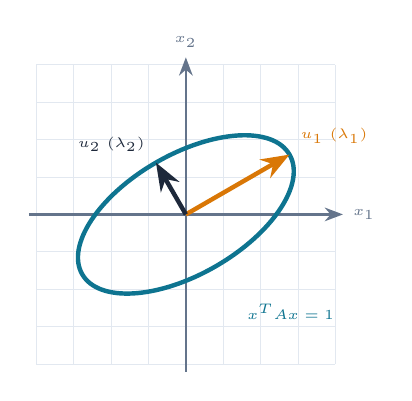
\begin{tikzpicture}[scale=0.95, >=Stealth]
          % Background Grid
          \draw[cardborder, step=0.5cm, line width=0.3pt] (-2.0,-2.0) grid (2.0,2.0);
          
          % Coordinate Axes
          \draw[->, slate, thick] (-2.1,0) -- (2.1,0) node[right, font=\tiny] {$x_1$};
          \draw[->, slate, thick] (0,-2.1) -- (0,2.1) node[above, font=\tiny] {$x_2$};
          
          % Rotated Ellipse (Level set x^T A x = 1)
          \draw[rotate around={30:(0,0)}, teal, ultra thick] (0,0) ellipse (1.6cm and 0.8cm);
          
          % Principal Eigenvector Axes
          \draw[rotate around={30:(0,0)}, ->, amber, ultra thick] (0,0) -- (1.6,0) node[above right, font=\tiny] {$u_1 \ (\lambda_1)$};
          \draw[rotate around={30:(0,0)}, ->, navy, ultra thick] (0,0) -- (0,0.8) node[above left, font=\tiny] {$u_2 \ (\lambda_2)$};
          
          % Label level set
          \node[teal, font=\tiny] at (1.4,-1.3) {$x^T A x = 1$};
        \end{tikzpicture}
      \end{center}
    \end{column}

    \begin{column}{0.48\textwidth}
      \begin{conceptbox}{Key Geometric Insights}
        \small
        \begin{itemize}
          \setlength{\itemsep}{3pt}
          \item Level sets $x^T A x = c$ for $A \succ 0$ are \hl{hyper-ellipsoids}.
          \item \textbf{Principal axes} align with orthogonal eigenvectors $u_1, \dots, u_n$.
          \item Semi-axis lengths equal $r_i = \frac{\sqrt{c}}{\sqrt{\lambda_i}}$.
        \end{itemize}
      \end{conceptbox}
    \end{column}
  \end{columns}
\end{frame}

% ==============================================================================
% SLIDE 16: Summary Table of Matrix Decompositions
% ==============================================================================
\begin{frame}{Matrix Factorization Summary}{Comparative Overview}
  \centering
  \footnotesize
  \begin{tabular}{llll}
    \toprule
    \rowcolor{cardbg}
    \textbf{Factorization} & \textbf{Applicable Matrices} & \textbf{Form} & \textbf{Key Properties} \\
    \midrule
    \textbf{Spectral} & Real Symmetric ($A=A^T$) & $A = Q \Lambda Q^T$ & $Q$ orthogonal, $\Lambda$ real diagonal \\{}
    [3pt]
    \textbf{SVD} & Any Rectangular ($m \times n$) & $A = U \Sigma V^T$ & $U, V$ orthogonal, $\Sigma \ge 0$ \\{}
    [3pt]
    \textbf{Cholesky} & Symmetric Pos-Def ($A \succ 0$) & $A = L L^T$ & $L$ lower triangular ($l_{ii} > 0$) \\{}
    [3pt]
    \textbf{QR} & Any Rectangular ($m \ge n$) & $A = Q R$ & $Q$ orthonormal, $R$ upper triangular \\
    \bottomrule
  \end{tabular}

  \vspace*{0.2cm}

  \begin{conceptbox}{Practical Data Science Applications}
    \small
    \begin{itemize}
      \setlength{\itemsep}{2pt}
      \item \textbf{Principal Component Analysis (PCA):} Diagonalize covariance matrix $C = \frac{1}{n} X^T X$.
      \item \textbf{Spectral Clustering:} Graph Laplacian eigenspace embedding $L = D - A$.
    \end{itemize}
  \end{conceptbox}
\end{frame}

% ==============================================================================
% SLIDE 17: Closing / Q&A Slide
% ==============================================================================
\begin{frame}[plain]
  \vspace*{1.2cm}
  \begin{center}
    {\color{teal}\small\bfseries THANK YOU FOR LISTENING} \\[0.2cm]
    {\color{navy}\huge\bfseries Questions \& Discussion} \\[0.3cm]
    
\begin{tikzpicture}
      \draw[amber, thick] (-1.5,0) -- (1.5,0);
    \end{tikzpicture}
    \par\vspace{0.4cm}
    
    \begin{conceptbox}{Next Lecture Preview}
      \centering
      \small
      \textbf{Lecture 8:} Singular Value Decomposition (SVD), Low-Rank Approximations, \\
      and the Eckart-Young-Mirsky Theorem.
    \end{conceptbox}
    
    \vspace*{0.3cm}
    {\color{slate}\small Contact: \code{a.mercer@nexa.edu} \quad$\cdot$\quad Office Hours: Wed 14:00--16:00}
  \end{center}
\end{frame}

\end{document}
